\documentclass[12pt,letterpaper,oneside]{book}

% ==============================================================================
% CORE PACKAGES & TYPOGRAPHY (PALATINO ENGINE - CONFLICT-FREE)
% ==============================================================================
\usepackage[utf8]{inputenc}
\usepackage[english]{babel}
\usepackage[T1]{fontenc}

% 1. Math packages (load amsmath FIRST)
\usepackage{amsmath}
\usepackage{bm}
% (Note: \usepackage{amssymb, amsfonts} removed — newpxmath provides all AMS symbols)

% 2. Palatino font suite
%\usepackage{newpxtext}
%\usepackage{newpxmath}

\usepackage[charter]{mathdesign}
\usepackage{XCharter}

\usepackage{microtype}
\usepackage{geometry}
\geometry{
    letterpaper,
    top=3.0cm,
    bottom=2.5cm,
    left=2.5cm,
    right=2.5cm,
    headheight=28pt
}
\usepackage{graphicx}
\usepackage{booktabs}
\usepackage{tabularx}
\usepackage{fancyhdr}
\usepackage{titlesec}
\usepackage{setspace}
\usepackage{cite}
\usepackage{url}
\usepackage{pdfpages}
\usepackage[colorlinks=true, linkcolor=blue, citecolor=blue, urlcolor=cyan]{hyperref}

% Body line spacing for doctoral thesis
\onehalfspacing

% ==============================================================================
% HEADERS & RUNNING PAGINATION (ONESIDE)
% ==============================================================================
\pagestyle{fancy}
\fancyhf{}
\fancyhead[R]{\small\thepage}
\fancyhead[L]{\small\nouppercase{\leftmark}}
\renewcommand{\headrulewidth}{0.4pt}
\renewcommand{\footrulewidth}{0pt}

\fancypagestyle{plain}{
    \fancyhf{}
    \fancyfoot[C]{\small\thepage}
    \renewcommand{\headrulewidth}{0pt}
}

% Chapter and Section Formats
\titleformat{\chapter}[display]
  {\normalfont\bfseries\LARGE}
  {\filleft\MakeUppercase{\chaptertitlename} \huge\thechapter}
  {2ex}
  {\titlerule\vspace{1.5ex}\filright}
  [\vspace{1.5ex}\titlerule]
\titlespacing*{\chapter}{0pt}{20pt}{30pt}

\titleformat*{\section}{\large\bfseries}
\titlespacing*{\section}{0pt}{18pt}{8pt}

\titleformat*{\subsection}{\normalsize\bfseries}
\titlespacing*{\subsection}{0pt}{12pt}{6pt}

% ==============================================================================
% DOCUMENT BEGINS
% ==============================================================================
\begin{document}

\frontmatter

% ------------------------------------------------------------------------------
% TITLE PAGE
% ------------------------------------------------------------------------------
\begin{titlepage}
\begin{center}
    \vspace*{0.5cm}
    {\LARGE \bfseries Development of an AI-Enhanced High-Fidelity Hybrid Semi-Symplectic Computational Framework for Massive Space Debris Fragmentation and Orbital Population Dynamics \par}
    
    \vspace{1.8cm}
    {\Large \textbf{Juan Francisco Puerta-Ibarra} \par}
    
    \vspace{2.0cm}
    {\normalsize Thesis presented as a partial requirement for the degree of: \\
    \textbf{Doctor of Philosophy (Ph.D.) in Engineering} \par}
    
    \vspace{2.0cm}
    {\normalsize
    \textbf{Advisors:} \\
    Nicolás Muñoz-Galeano, Ph.D. (Director) \\
    Bonnie Prado Pino, Ph.D. (Co-Advisor) \par}
    
    \vfill
    {\normalsize
    Faculty of Engineering \\
    Department of Mechanical and Aerospace Engineering \\
    Research Group in Efficient Energy Management (GIMEL) \\
    Universidad de Antioquia \\
    Medellín, Colombia \\
    2026 \par}
\end{center}
\end{titlepage}

\clearpage

% ------------------------------------------------------------------------------
% PRELIMINARY PAGES
% ------------------------------------------------------------------------------
\tableofcontents
\listoffigures
\listoftables

\clearpage

% ==============================================================================
% MAIN BODY (COMPENDIUM MODULES)
% ==============================================================================
\mainmatter

% Chapter 1: Comprehensive Introduction & Synthesis (Swales CARS Model)
\chapter{Introduction}
\label{ch:introduction}

% ==============================================================================
% MOVE 1: ESTABLISHING A TERRITORY (WHAT IS KNOWN)
% ==============================================================================
\section{Global Context and Operational Relevance}
\label{sec:context}

The emergence of the ``NewSpace'' commercial paradigm transforms access to near-Earth space. This shift accelerates the deployment of commercial mega-constellations, standardized small satellites, and multi-payload launch missions. While this orbital expansion enables global telecommunications, precision Earth observation, and scientific services, it drives Low Earth Orbit (LEO)---spanning altitudes between 200~km and 2,000~km---toward critical operational saturation. Global Space Situational Awareness (SSA) tracking registries indicate that more than 35,000 anthropogenic debris objects larger than 10~cm are routinely cataloged \cite{anz-meador_assessment_2004}. Simultaneously, statistical environmental models estimate that an untracked population exceeding 500,000 lethal fragments with characteristic lengths between 1~cm and 10~cm circulates within the same orbital regime. Orbital velocities in LEO average between 7.5~km/s and 7.8~km/s. Consequently, hypervelocity impacts with millimeter- or centimeter-scale debris release kinetic energy sufficient to disable operational spacecraft.

Catastrophic fragmentation events serve as the primary drivers of discrete orbital population surges \cite{anz-meador_assessment_2004}. These events arise from upper-stage propulsion explosions, battery over-pressurizations, accidental hypervelocity collisions, and deliberate kinetic Anti-Satellite (ASAT) engagements. Landmark historical incidents, notably the 2007 Fengyun-1C kinetic engagement and the 2009 hypervelocity collision between Iridium~33 and Cosmos~2251, injected thousands of long-lived fragments across wide altitude and inclination bands. These events demonstrate that collision fragments rapidly disperse into concentric shells that intersect vital commercial and scientific orbits. Left unmitigated, this exponential debris growth threatens to trigger the Kessler syndrome \cite{kessler_collision_1978}. This phenomenon is a self-sustaining collisional cascade. In this scenario, the rate of impact-driven fragment generation surpasses the rate of natural orbital decay induced by atmospheric drag \cite{kessler_collision_1978}.

At both global and national levels, the preservation of the LEO environment represents an urgent engineering priority. Internationally, agencies such as the National Aeronautics and Space Administration (NASA) and the European Space Agency (ESA) mandate strict Space Traffic Management (STM) protocols and post-mission disposal guidelines. Regionally, emerging aerospace nations in Latin America increasingly rely on LEO assets for environmental monitoring, territorial sovereignty, and disaster management. In Colombia, this development is led by university CubeSat missions, the Colombian Air and Space Force (FAC) Earth observation programs, and academic research centers such as the Universidad de Antioquia. However, regional operators and global researchers alike face a severe computational barrier. Predicting the multi-decade evolution of massive debris clouds typically requires supercomputing infrastructure that remains inaccessible to standard astrodynamics laboratories. Therefore, developing mathematically rigorous and computationally efficient orbital propagation frameworks is essential to democratize high-fidelity SSA and ensure long-term orbital sustainability.

\section{State of the Art in Orbital Debris Modeling and Propagation}
\label{sec:sota}

The scientific literature establishes several methodological paradigms to initialize, propagate, and screen orbital fragmentation clouds. To characterize the initial state of a breakup event, statistical empirical formulations such as the NASA Standard Breakup Model (SBM), originally implemented in the EVOLVE 4.0 framework \cite{johnson_nasas_2001}, and the ESA MASTER model define probability distributions for fragment characteristic length ($L_c$), Area-to-Mass ratio ($A/m$), and ejection velocity ($\Delta v$). Once initialized, forecasting the spatial and temporal evolution of these fragments relies on three primary propagation approaches: analytical theories, explicit numerical integrators, and geometric structure-preserving schemes.

Analytical and semi-analytical propagators, most notably the Simplified General Perturbations-4 (SGP4) model coupled with Two-Line Element (TLE) sets, use closed-form secular and periodic approximations of Earth's oblateness ($J_2$--$J_4$) and simplified atmospheric drag. This formulation achieves rapid execution speeds for routine catalog maintenance. Conversely, mission-critical trajectory design relies on high-order explicit numerical integration schemes. These include explicit Runge-Kutta (RK) methods, Dormand-Prince (RK8) solvers, and Cowell formulations implemented in standard software suites such as NASA's General Mission Analysis Tool (GMAT), Ansys Systems Tool Kit (STK), and ESA's GODOT. These explicit solvers evaluate complex perturbation accelerations at each integration step, including high-degree spherical harmonics, empirical thermospheric density models (such as NRLMSISE-00 and Jacchia-Roberts), and Solar Radiation Pressure (SRP).

In the domain of long-term celestial mechanics, symplectic integrators represent the gold standard for conservative Hamiltonian systems \cite{sanz-serna_symplectic_1992}. Grounded in the Wisdom-Holman mapping and popularized through the C-based REBOUND library \cite{ReinLiu2012} via the Wisdom-Holman Fast (WHFast) algorithm \cite{rein_whfast_2015}, symplectic integrators preserve the canonical phase-space volume ($d\mathbf{p} \wedge d\mathbf{q}$). Rather than accumulating unbounded truncation errors, a symplectic integrator of order $r$ operating at a fixed step size $\Delta t$ exactly solves a shadow Hamiltonian $H_\infty = H + \mathcal{O}(\Delta t^r)$. This property bounds global mechanical energy oscillations indefinitely \cite{sanz-serna_symplectic_1992, rein_whfast_2015}. Recent extensions within the past decade, such as the REBOUNDx library and operator-splitting schemes based on Strang splitting, demonstrate that non-conservative perturbations can be coupled with symplectic cores by alternating conservative drift steps with perturbative velocity kicks.

\subsection{Artificial Intelligence and Machine Learning in Computational Astrodynamics}
\label{sec:sota_ai}

Over the past decade, the rapid maturation of Scientific Machine Learning (SciML) and Artificial Intelligence (AI) introduces data-driven paradigms that complement and accelerate classical numerical astrodynamics. Rather than functioning purely as empirical black-box regressors, modern architectures embed fundamental physical principles, geometric spatial partitioning, and decision-making formalisms directly into computational pipelines:

\paragraph{Physics-Informed Neural Networks (PINNs):}
PINNs solve forward and inverse problems governed by differential equations by embedding physical laws directly into the neural network loss function as soft regularization constraints \cite{raissi_physics-informed_2019}. Using exact Automatic Differentiation (AD) via backpropagation through the computational graph, PINNs evaluate spatial and temporal derivatives to machine precision without requiring discrete computational grids or finite-difference stencils \cite{raissi_physics-informed_2019}. In atmospheric flight dynamics and astrodynamics, PINNs provide continuous, smooth surrogates for volatile thermospheric density fields. They effectively replace traditional discrete look-up tables and empirical models that introduce non-physical gradient discontinuities.

\paragraph{Spatial Partitioning and Sequential Conjunction Classifiers:}
Operational conjunction assessment across expanding orbital swarms presents an acute computational challenge. Spatial decomposition structures, particularly $K$-Dimensional Trees (KD-Trees), recursively bisect multi-dimensional Euclidean coordinate spaces along alternating orthogonal planes. This partitioning transforms all-on-all pairwise neighbor searches from quadratic complexity down to logarithmic scaling. Concurrently, deep recurrent sequence models, specifically Long Short-Term Memory (LSTM) networks, capture long-range temporal dependencies within relative trajectory states. By regulating information flow through input, forget, and output gating mechanisms, LSTMs accurately classify hyperbolic miss-distance vectors. They also forecast close approaches under severe class imbalances, where benign flybys outnumber true collision events by orders of magnitude.

\paragraph{Reinforcement Learning (RL) and Markov Decision Processes (MDPs):}
Reinforcement learning formulates complex trajectory optimization and inverse estimation tasks as Markov Decision Processes, defined by the tuple $(\mathcal{S}, \mathcal{A}, \mathcal{P}, \mathcal{R}, \gamma)$. Policy gradient algorithms, particularly Proximal Policy Optimization (PPO), maintain stable policy updates in continuous state and action spaces through clipped surrogate objective functions. These clipped objectives prevent destructively large gradient steps during training. When applied to astrodynamic inverse targeting, PPO agents learn optimal exploration strategies across perturbed orbital manifolds, identifying the origin state of historical fragmentation events from downstream orbital tracking observations.

Table~\ref{tab:sota_synthesis} synthesizes the primary methodological approaches reported in the literature for orbital propagation and debris analysis.

\begin{table}[htbp]
\centering
\caption{Synthesis of orbital propagation and debris analysis methodologies in the literature.}
\label{tab:sota_synthesis}
\begin{spacing}{1.08}
\small
\begin{tabularx}{\textwidth}{
    >{\raggedright\arraybackslash}p{2.8cm}
    >{\raggedright\arraybackslash}p{3.6cm}
    >{\raggedright\arraybackslash}p{3.1cm}
    >{\raggedright\arraybackslash}X
}
\toprule
\textbf{Methodology / Tool} & \textbf{Core Formulation} & \textbf{Energy Behavior} & \textbf{Primary Operational Scope} \\
\midrule
SGP4 / TLE & Analytical perturbation theory & Approximate / Secular decay & Fast catalog maintenance; low precision over multi-week arcs. \\
\addlinespace[0.4em]
Cowell / RK8 (GMAT, STK) & High-order explicit numerical integration & Unbounded secular truncation drift & High-precision single-satellite mission design; slow for $N > 10^4$. \\
\addlinespace[0.4em]
Wisdom-Holman / WHFast \cite{rein_whfast_2015} & Canonical symplectic splitting & Strictly bounded ($\mathcal{O}(\Delta t^r)$) & Multi-decade conservative planetary $N$-body dynamics. \\
\addlinespace[0.4em]
Operator Splitting (REBOUNDx) & Symmetric kick-drift-kick composition & Bounded adiabatic invariants & Weakly perturbed celestial systems; limited LEO drag validation. \\
\addlinespace[0.4em]
AI/ML Surrogates (PINN \cite{raissi_physics-informed_2019}, LSTM, RL) & Neural function approximation and spatial indexing & Data- and physics-regularized & Differentiable atmospheric modeling, $\mathcal{O}(N \log N)$ conjunction screening, and inverse targeting. \\
\bottomrule
\end{tabularx}
\end{spacing}
\end{table}

% ==============================================================================
% MOVE 2: ESTABLISHING A NICHE (CONTRAST + GAP + CONSEQUENCE)
% ==============================================================================
\section{Critical Evaluation of Existing Knowledge and Research Gaps}
\label{sec:niche}

Despite substantial progress in individual propagation algorithms and machine learning surrogates, a critical evaluation of the state of the art reveals that existing computational frameworks remain insufficient. Current methods cannot simultaneously satisfy the physical fidelity, long-term numerical stability, and computational scalability required to model massive LEO fragmentation events ($N \ge 50,000$). Following a systematic evaluation of the literature, three fundamental research gaps persist:

\paragraph{1. Methodological Limitation in Massive Multi-Decade Integrations (Truncation Drift vs.\ Scalability):}
Classical astrodynamics software suites rely on explicit numerical integrators, such as RK8 and Cowell formulations, to achieve high local accuracy. However, explicit schemes do not preserve the underlying geometric invariants of orbital mechanics, causing local truncation errors to accumulate monotonically over thousands of revolutions. Conversely, while analytical SGP4 propagators scale rapidly, they omit higher-order nonlinear coupling and fail to maintain sub-kilometer deterministic accuracy following high-energy breakup events. Consequently, long-term numerical simulations suffer from artificial secular energy drift---manifesting as non-physical orbital contraction or expansion---and incur prohibitive computational runtimes when scaling to clouds exceeding $N = 20,000$ fragments, rendering multi-decade population forecasting intractable for standard astrodynamics laboratories.

\paragraph{2. Theoretical Gap in Non-Conservative Dissipative Symplectic Propagation:}
While symplectic integrators such as WHFast \cite{rein_whfast_2015} eliminate secular energy drift in conservative gravitational fields, their mathematical derivation strictly requires a time-invariant Hamiltonian system. However, the LEO environment is governed by non-Hamiltonian, velocity-dependent dissipative forces---principally atmospheric drag and SRP---which continuously contract phase-space volume and violate canonical symplectic invariants. Existing workarounds either abandon the symplectic structure entirely or apply adaptive time-stepping schemes that destroy the shadow Hamiltonian and reintroduce quadratic error growth. Consequently, a critical gap remains in formulating and validating a constant-time-step, second-order symmetric Strang splitting architecture that couples Earth's zonal geopotential harmonics ($J_2, J_4$) with drag and SRP across 50,000 debris fragments without degrading secular angular momentum invariants.

\paragraph{3. Computational Bottlenecks in Atmospheric Evaluation, Conjunction Screening, and Inverse Reconstruction:}
Even when a stable semi-symplectic integrator is established, operationalizing the framework for STM encounters three severe latency bottlenecks:
\begin{itemize}
    \item First, standard piecewise-exponential atmospheric look-up tables contain spatial gradient discontinuities ($\mathcal{C}^0$) at altitude boundaries. These discontinuities inject artificial numerical noise into fixed-step symplectic velocity kicks, whereas full empirical models (NRLMSISE-00) are computationally prohibitive to evaluate $5 \times 10^4$ times per time step.
    \item Second, evaluating close approaches across $N$ dispersing fragments via brute-force pairwise checking incurs a quadratic computational complexity of $\mathcal{O}(N^2)$. This approach requires $1.25 \times 10^9$ distance evaluations per time step for $N = 50,000$, which stalls real-time collision forecasting.
    \item Third, solving the inverse astrodynamics problem---reconstructing historical breakup coordinates and epochs from dispersed orbital observations---requires thousands of iterative simulation rollouts. In conventional architectures, exchanging state vectors between compiled propagation engines and high-level optimization scripts relies on disk Input/Output (I/O) serialization, creating a severe data-transfer bottleneck.
\end{itemize}
Consequently, these combined computational latencies prevent regional aerospace agencies and academic operators from executing real-time conjunction screening and autonomous fragmentation reconstruction, leaving operational LEO satellites vulnerable to uncataloged debris swarms.

\subsection{Research Questions}
\label{subsec:research_questions}

To address the identified methodological limitations and theoretical gaps, this doctoral research formulates the following overarching and specific research questions:

\begin{itemize}
    \item \textbf{General Research Question:} How can structure-preserving symplectic integration be mathematically coupled with non-conservative environmental perturbations and embedded artificial intelligence architectures to enable high-fidelity, scalable Orbital Population Dynamics forecasting and autonomous fragmentation reconstruction for massive space debris clouds ($N \ge 50,000$) in Low Earth Orbit?
    \item \textbf{Specific Research Question 1:} To what extent does a fixed-step WHFast symplectic $N$-body formulation preserve mechanical energy bounds and positional accuracy relative to industry-standard explicit propagators when scaling to $N = 20,000$ fragments under Earth's $J_2$ and $J_4$ zonal geopotential harmonics?
    \item \textbf{Specific Research Question 2:} How effectively does a symmetric second-order Strang operator splitting scheme ($\Phi_P(\Delta t/2) \circ \Phi_G(\Delta t) \circ \Phi_P(\Delta t/2)$) integrate non-conservative atmospheric drag and Solar Radiation Pressure across $N = 50,000$ fragments without degrading conservative secular nodal precession invariants?
    \item \textbf{Specific Research Question 3:} How can embedded Physics-Informed Neural Networks, spatial KD-Tree partitioning with LSTM sequence classifiers, and shared-memory Reinforcement Learning agents eliminate thermospheric gradient discontinuities, reduce $\mathcal{O}(N^2)$ conjunction screening complexity, and resolve disk I/O bottlenecks during inverse breakup reconstruction?
\end{itemize}

% ==============================================================================
% MOVE 3: OCCUPYING THE NICHE (THE PROPOSED SOLUTION)
% ==============================================================================
\section{Proposed Computational Framework and Scope}
\label{sec:occupying_niche}

To resolve the aforementioned challenges, this study proposes an AI-enhanced, high-fidelity hybrid semi-symplectic computational framework for massive LEO debris cloud propagation, conjunction assessment, and inverse event reconstruction. The proposed methodology integrates a compiled C-based symplectic core (adapted from REBOUND's WHFast solver \cite{ReinLiu2012, rein_whfast_2015}) with a symmetric second-order Strang operator splitting sequence and a three-tier embedded AI ecosystem in Python.

The analysis is conducted using synthetic fragmentation populations of $N = 20,000$ to $N = 50,000$ autonomous debris objects procedurally generated via the NASA Standard Breakup Model (SBM) \cite{johnson_nasas_2001}. These populations incorporate realistic distributions of characteristic lengths, area-to-mass ratios ($A/m$), and ejection velocities. Trajectory fidelity and secular orbital invariants are cross-validated against analytical perturbation theory and NASA's General Mission Analysis Tool (GMAT vR2025a). Unlike prior studies that treat numerical propagation, atmospheric modeling, and machine learning as isolated offline tasks, this framework embeds neural surrogates and reinforcement learning directly into the compiled integration loop via a zero-copy \texttt{ctypes} shared-memory pointer bridge. This integrated approach unifies structure-preserving astrodynamics with scientific machine learning, enabling deterministic multi-decade debris forecasting on standard workstation hardware. The scope of the study encompasses perturbed Low Earth Orbit regimes (altitudes between 200~km and 2,000~km) governed by central gravity, $J_2$ and $J_4$ zonal harmonics, atmospheric drag, and Solar Radiation Pressure.

\subsection{Three-Tier Embedded AI Ecosystem Architecture}
\label{subsec:three_tier_ai}

To dismantle the computational bottlenecks identified in Section~\ref{sec:niche}, the framework embeds three synergistic AI tiers directly within the numerical integration pipeline:

\paragraph{Tier 1 --- Hydrostatic Physics-Informed Neural Network (PINN) Surrogate:}
The first tier eliminates the high-frequency numerical chattering and step-size truncation spikes caused by $\mathcal{C}^0$ gradient discontinuities in piecewise-exponential lookup tables. A feedforward neural network $\mathcal{N}_\theta: h \to \hat{\rho}$ parameterized by weights $\theta$ acts as an analytical surrogate for thermospheric density \cite{raissi_physics-informed_2019}. Rather than fitting observational data in an unconstrained manner, the network is strictly regularized by the differential equation of hydrostatic equilibrium governing scale-height atmospheric decay:
\begin{equation}
\frac{d\rho}{dh} = -\frac{\rho(h)}{H(h)}
\label{eq:hydrostatic_ode}
\end{equation}
where $h$ denotes geodetic altitude and $H(h)$ represents the localized thermospheric scale height. The composite loss function minimized during training is formulated as:
\begin{equation}
\mathcal{L}_{\text{Total}}(\theta) = \mathcal{L}_{\text{Data}}(\theta) + \lambda \mathcal{L}_{\text{Physics}}(\theta)
\label{eq:pinn_total_loss}
\end{equation}
with the physics residual penalty defined across $N_c$ collocation points:
\begin{equation}
\mathcal{L}_{\text{Physics}}(\theta) = \frac{1}{N_c} \sum_{j=1}^{N_c} \left\| \frac{d\mathcal{N}_\theta(h_j)}{dh} + \frac{\mathcal{N}_\theta(h_j)}{H(h_j)} \right\|^2
\label{eq:pinn_physics_residual}
\end{equation}
The derivative $d\mathcal{N}_\theta / dh$ is evaluated to machine precision via automatic differentiation across the network's computational graph. This architecture establishes a smooth, $\mathcal{C}^\infty$-differentiable density manifold across LEO altitudes (100~km to 2,000~km), stabilizing the velocity kicks within the Strang splitting sequence and accelerating aerodynamic drag evaluations.

\paragraph{Tier 2 --- Spatial KD-Tree Domain Decomposition and LSTM Conjunction Screening:}
The second tier bypasses the quadratic $\mathcal{O}(N^2)$ computational barrier of all-on-all pairwise proximity screening across $N = 50,000$ fragments. It decouples global orbital propagation from proximity assessment using a two-stage geometric and sequential pipeline:
\begin{enumerate}
    \item \textit{Geometric Manifold Pruning via KD-Trees:} At each integration step $\Delta t$, a three-dimensional $K$-Dimensional Tree recursively partitions the Cartesian position coordinates $\mathbf{r} = [x, y, z]^T \in \mathbb{R}^3$ of the entire fragment population along alternating orthogonal median planes. For any primary asset $\mathbf{r}_{\text{target}}$, the KD-Tree executes a localized hyperspherical query filtering for candidate debris particles $j$ satisfying:
    \begin{equation}
    d(\mathbf{r}_{\text{target}}, \mathbf{r}_j) = \|\mathbf{r}_{\text{target}} - \mathbf{r}_j\|_2 \le R_{\text{filter}}
    \label{eq:kdtree_filter}
    \end{equation}
    where $R_{\text{filter}} = 50$~km denotes a conservative screening envelope. This spatial decomposition reduces proximity search complexity from $\mathcal{O}(N^2)$ to $\mathcal{O}(N \log N)$, pruning millions of benign orbital pairings before deep learning ingestion.
    \item \textit{Kinematic Sequence Classification via LSTM:} Proximal fragment pairs ($k \ll N$) are structured into historical time-series sequences of 6D relative Cartesian states $\mathbf{x}_k = [\Delta \mathbf{r}_k, \Delta \mathbf{v}_k]^T \in \mathbb{R}^6$. An LSTM recurrent network processes these sequences through its gating architecture:
    \begin{align}
    \mathbf{i}_k &= \sigma(\mathbf{W}_i \mathbf{x}_k + \mathbf{U}_i \mathbf{h}_{k-1} + \mathbf{b}_i) \label{eq:lstm_i} \\
    \mathbf{f}_k &= \sigma(\mathbf{W}_f \mathbf{x}_k + \mathbf{U}_f \mathbf{h}_{k-1} + \mathbf{b}_f) \label{eq:lstm_f} \\
    \mathbf{c}_k &= \mathbf{f}_k \odot \mathbf{c}_{k-1} + \mathbf{i}_k \odot \tanh(\mathbf{W}_c \mathbf{x}_k + \mathbf{U}_c \mathbf{h}_{k-1} + \mathbf{b}_c) \label{eq:lstm_c} \\
    \mathbf{o}_k &= \sigma(\mathbf{W}_o \mathbf{x}_k + \mathbf{U}_o \mathbf{h}_{k-1} + \mathbf{b}_o) \label{eq:lstm_o} \\
    \mathbf{h}_k &= \mathbf{o}_k \odot \tanh(\mathbf{c}_k) \label{eq:lstm_h}
    \end{align}
    where $\sigma$ denotes the sigmoid activation function and $\odot$ represents the Hadamard product. The terminal hidden state $\mathbf{h}_t$ outputs a continuous collision warning probability $\hat{y}_t \in [0, 1]$ optimized via Binary Cross-Entropy (BCE) loss. This recurrent formulation captures subtle variations in non-conservative energy decay, achieving 100\% recall across high-risk conjunction arcs under severe class imbalance.
\end{enumerate}

\paragraph{Tier 3 --- In-Memory PPO Reinforcement Learning for Inverse Breakup Targeting:}
The third tier resolves the non-convex inverse astrodynamics problem of identifying the historical epoch ($t_0$), Cartesian coordinates, and ejection energy of an uncataloged fragmentation event from sparse downstream cloud observations. Rather than relying on disk-bound simulation files that introduce severe I/O bottlenecks, the inverse task is cast as a continuous Markov Decision Process and solved via Proximal Policy Optimization:
\begin{itemize}
    \item \textit{Action Space ($\mathbf{a}_t \in \mathbb{R}^5$):} The policy generates continuous perturbation vectors modifying the candidate breakup parameters:
    \begin{equation}
    \mathbf{a}_t = [\delta t, \, \delta x, \, \delta y, \, \delta z, \, \delta v_{\text{spread}}]^T
    \label{eq:ppo_action}
    \end{equation}
    where $\delta t$ represents the temporal shift, $[\delta x, \delta y, \delta z]$ are Cartesian origin coordinates, and $\delta v_{\text{spread}}$ modulates the isotropic ejection velocity dispersion magnitude.
    \item \textit{State Space ($\mathbf{s}_t \in \mathbb{R}^{12}$):} The observation vector provided to the policy captures the first and second statistical moments of the debris cloud relative to observational tracking data:
    \begin{equation}
    \mathbf{s}_t = [\boldsymbol{\mu}_{\text{sim}} - \boldsymbol{\mu}_{\text{obs}}, \, \boldsymbol{\sigma}_{\text{sim}} - \boldsymbol{\sigma}_{\text{obs}}]^T
    \label{eq:ppo_state}
    \end{equation}
    where $\boldsymbol{\mu} = [\bar{x}, \bar{y}, \bar{z}]^T$ is the cloud centroid and $\boldsymbol{\sigma} = [\sigma_x, \sigma_y, \sigma_z]^T$ represents spatial standard deviation.
    \item \textit{Reward Formulation ($R_t$):} To steer the agent toward the true breakup origin without requiring point-to-point debris matching, the reward function minimizes macroscale distributional divergence:
    \begin{equation}
    R_t = -\frac{1}{C} \sqrt{ \|\boldsymbol{\mu}_{\text{sim}} - \boldsymbol{\mu}_{\text{obs}}\|_2^2 + \|\boldsymbol{\sigma}_{\text{sim}} - \boldsymbol{\sigma}_{\text{obs}}\|_2^2 }
    \label{eq:ppo_reward}
    \end{equation}
    where $C \in \mathbb{R}^+$ is a standardizing scaling parameter.
    \item \textit{Shared-Memory Pointer Bridge:} The policy network is optimized using the clipped surrogate objective $L^{\text{CLIP}}(\theta)$. To bypass file serialization entirely, the compiled C symplectic propagation engine (\texttt{rl\_propagator.so}) links directly into Python Gymnasium rollout workers via a zero-copy \texttt{ctypes} shared-memory pointer interface. This shared-RAM architecture executes 32,768-step rollout blocks at 37 frames per second (FPS) across 16 CPU cores, optimizing historical breakup parameters entirely in random-access memory.
\end{itemize}

\section{Research Objectives and Methodological Alignment}
\label{sec:objectives}

\subsection{General Objective}
The general objective of this study is to develop, validate, and optimize an AI-enhanced high-fidelity hybrid semi-symplectic computational framework capable of modeling massive space debris fragmentation and long-term population dynamics within non-conservative orbital environments to support space traffic management and space sustainability operations.

\subsection{Specific Objectives}
\begin{enumerate}
    \item \textbf{Specific Objective 1:} Develop and mathematically verify a scalable symplectic $N$-body propagation core capable of modeling Earth's conservative geopotential field ($J_2, J_4$) for massive debris clouds ($N \ge 20,000$) with bounded numerical energy drift.
    \item \textbf{Specific Objective 2:} Formulate and implement a symmetric second-order Strang operator splitting integration scheme that couples conservative Hamiltonian gravity with non-conservative perturbations (piecewise-exponential atmospheric drag and Solar Radiation Pressure) across populations of 50,000 fragments.
    \item \textbf{Specific Objective 3:} Integrate embedded deep learning and reinforcement learning models (PINN thermospheric surrogate, KD-Tree/LSTM conjunction classifier, and shared-memory PPO agent) to resolve computational latencies in thermospheric density evaluation, close-approach conjunction mapping, and inverse fragmentation event reconstruction.
\end{enumerate}

In accordance with doctoral research design guidelines, each specific objective corresponds directly to a dedicated methodological formulation, a quantitative set of validation results, and a critical discussion block within the compendium chapters, as detailed in Table~\ref{tab:objective_alignment}.

\begin{table}[htbp]
\centering
\caption{Alignment of Specific Objectives with Methods, Results, and Discussion chapters.}
\label{tab:objective_alignment}
\footnotesize
\begin{tabularx}{\textwidth}{l X X l}
\toprule
\textbf{Objective} & \textbf{Methodological Component (Methods)} & \textbf{Key Validation Metrics (Results)} & \textbf{Compendium Location (Discussion)} \\
\midrule
\textbf{Objective 1} & WHFast symplectic solver in Jacobi/democratic heliocentric coordinates with $J_2, J_4$ zonal potentials. & Sub-km agreement vs.\ NASA GMAT; energy error $|\Delta E/E_0| \in [10^{-8}, 10^{-7}]$; scaling $\mathcal{O}(N^{1.60})$ for $N = 20,000$. & Chapter~\ref{ch:paper1} (Paper 1: AAS 25-787 \cite{puerta-ibarra_aas25_2025}) \\
\addlinespace
\textbf{Objective 2} & Symmetric 2nd-order Strang splitting $\Phi_P(\Delta t/2) \circ \Phi_G(\Delta t) \circ \Phi_P(\Delta t/2)$ at constant $\Delta t = 10$~s with NASA SBM initialization. & Nodal precession error $< 0.005\%$ vs.\ analytical theory; verified $A/m$ orbital sorting across $N = 50,000$. & Chapter~\ref{ch:paper2} (Paper 2: Strang Splitting) \\
\addlinespace
\textbf{Objective 3} & Hydrostatic-regularized PINN ($\mathcal{C}^\infty$); spatial KD-Tree + LSTM classifier; C-to-Python \texttt{ctypes} bridge + 16-core PPO MDP agent. & Smooth density gradients; $\mathcal{O}(N \log N)$ search; 100\% recall on 702 conjunction arcs; 37~FPS in-RAM inverse reconstruction. & Chapter~\ref{ch:paper3} (Paper 3: AAS 26-993 \cite{puerta-ibarra_aas26_2026}) \\
\bottomrule
\end{tabularx}
\end{table}

\section{Main Scientific Contributions}
\label{sec:contributions}

This doctoral dissertation advances the field of computational astrodynamics and Space Traffic Management through three primary scientific contributions:
\begin{itemize}
    \item \textbf{Contribution 1 --- Validated Symplectic Geopotential Baseline (Chapter~\ref{ch:paper1}):} Published in the \textit{AAS/AIAA Astrodynamics Specialist Conference} (Paper AAS 25-787) \cite{puerta-ibarra_aas25_2025}, this work demonstrates that a structure-preserving WHFast symplectic $N$-body architecture propagates 20,000 LEO fragments under $J_2$ and $J_4$ perturbations with sub-kilometer consistency relative to NASA's GMAT. The formulation bounds relative mechanical energy error within $|\Delta E/E_0| \le 10^{-7}$ and establishes a predictable power-law scalability exponent of 1.60.
    \item \textbf{Contribution 2 --- Second-Order Strang Splitting Semi-Symplectic Architecture (Chapter~\ref{ch:paper2}):} This research formulates a constant-step ($\Delta t = 10$~s) symmetric Strang splitting sequence that decouples conservative Hamiltonian geopotential drift from half-step dissipative drag and SRP kicks. Scaled to 50,000 SBM fragments, the solver preserves secular nodal precession within 0.005\% of analytical perturbation theory and captures physical ``orbital sorting'' driven by fragment area-to-mass ratios ($A/m$).
    \item \textbf{Contribution 3 --- Embedded Multi-Tier AI Ecosystem for Conjunction Screening and Inverse Targeting (Chapter~\ref{ch:paper3}):} Published in the \textit{AAS/AIAA Astrodynamics Specialist Conference} (Paper AAS 26-993) \cite{puerta-ibarra_aas26_2026}, this stage embeds three synergistic AI/ML modules directly into the symplectic loop: (i) a $\mathcal{C}^\infty$-differentiable PINN thermospheric surrogate governed by hydrostatic equilibrium that eliminates lookup table gradient spikes; (ii) a spatial KD-Tree and LSTM sequence classifier that reduces pairwise conjunction screening complexity from $\mathcal{O}(N^2)$ to $\mathcal{O}(N \log N)$ while achieving 100\% classification accuracy across 702 high-risk collision arcs; and (iii) an in-memory C-to-Python (\texttt{ctypes}) PPO reinforcement learning agent that executes 32,768-step MDP rollouts in Random-Access Memory (RAM) at 37~FPS across 16 CPU cores to autonomously reconstruct historical fragmentation coordinates.
\end{itemize}

\section{Thesis Organization}
\label{sec:organization}

The remainder of this compendium dissertation is organized into four subsequent chapters:
\begin{itemize}
    \item \textbf{Chapter~\ref{ch:paper1}} presents the formulation, implementation, and GMAT cross-validation of the conservative symplectic $N$-body baseline for 20,000 LEO debris fragments (Paper AAS 25-787) \cite{puerta-ibarra_aas25_2025}.
    \item \textbf{Chapter~\ref{ch:paper2}} develops the symmetric second-order Strang operator splitting framework, detailing the mathematical coupling of conservative geopotential harmonics with dissipative atmospheric drag and Solar Radiation Pressure across 50,000 fragments.
    \item \textbf{Chapter~\ref{ch:paper3}} details the design, training, and hardware-level integration of the embedded PINN thermospheric surrogate, the KD-Tree/LSTM conjunction assessment pipeline, and the shared-memory PPO reinforcement learning agent for inverse breakup reconstruction (Paper AAS 26-993) \cite{puerta-ibarra_aas26_2026}.
    \item \textbf{Chapter~\ref{ch:conclusions}} synthesizes the general and specific conclusions of the doctoral research, evaluates the fulfillment of the research objectives, and outlines strategic directions for future investigation in High-Performance Computing (HPC) and cislunar astrodynamics.
\end{itemize}

% Chapter 2: Publication 1 (AAS 25-787 / Symplectic Baseline)
% ------------------------------------------------------------------------------
% CHAPTER 2: PAPER 1 (AAS 25-787)
% ------------------------------------------------------------------------------
\chapter{Advanced Modeling Techniques for Analyzing Space Debris Fragmentation and Evolution}
\chaptermark{Symplectic Debris Fragmentation Modeling}
\label{ch:paper1}

\section*{Chapter Overview and Contextualization}
This chapter addresses the first specific objective of this doctoral research by developing and validating a structure-preserving $N$-body propagation framework for high-density space debris environments. This chapter synthesizes and presents the research published in the \textit{AAS/AIAA Astrodynamics Specialist Conference} (Paper AAS 25-787).

Predicting the evolutionary trajectory of fragmentation clouds requires maintaining numerical stability across millions of integration steps. Traditional explicit numerical propagators (e.g., standard Runge-Kutta or Cowell formulations) suffer from the accumulation of truncation errors, which manifest as non-physical secular drifts in mechanical energy. This chapter evaluates the application of symplectic integration schemes---specifically the WHFast symplectic $N$-body solver from the REBOUND library---to model the motion of 20,000 autonomous fragments under Earth's central gravity and zonal geopotential harmonics ($J_2$ and $J_4$).

The primary contribution of this work lies in proving that symplectic $N$-body formulations maintain bounded relative energy errors ($|\Delta E/E_0| \le 10^{-7}$) over extended propagation windows while delivering sub-kilometer orbital element consistency when benchmarked against NASA's General Mission Analysis Tool (GMAT). Furthermore, computational scalability tests demonstrate that the architecture follows a predictable power-law scaling exponent of 1.60, establishing the numerical baseline required for the subsequent integration of dissipative environmental perturbations.

\newpage
% \includepdf[pages=-, scale=0.95, pagecommand={\thispagestyle{plain}}]{papers/AAS_25_787.pdf}

\clearpage

% Check if the compiled PDF exists; embed if found, display placeholder if missing
\IfFileExists{papers/paper1.pdf}{%
    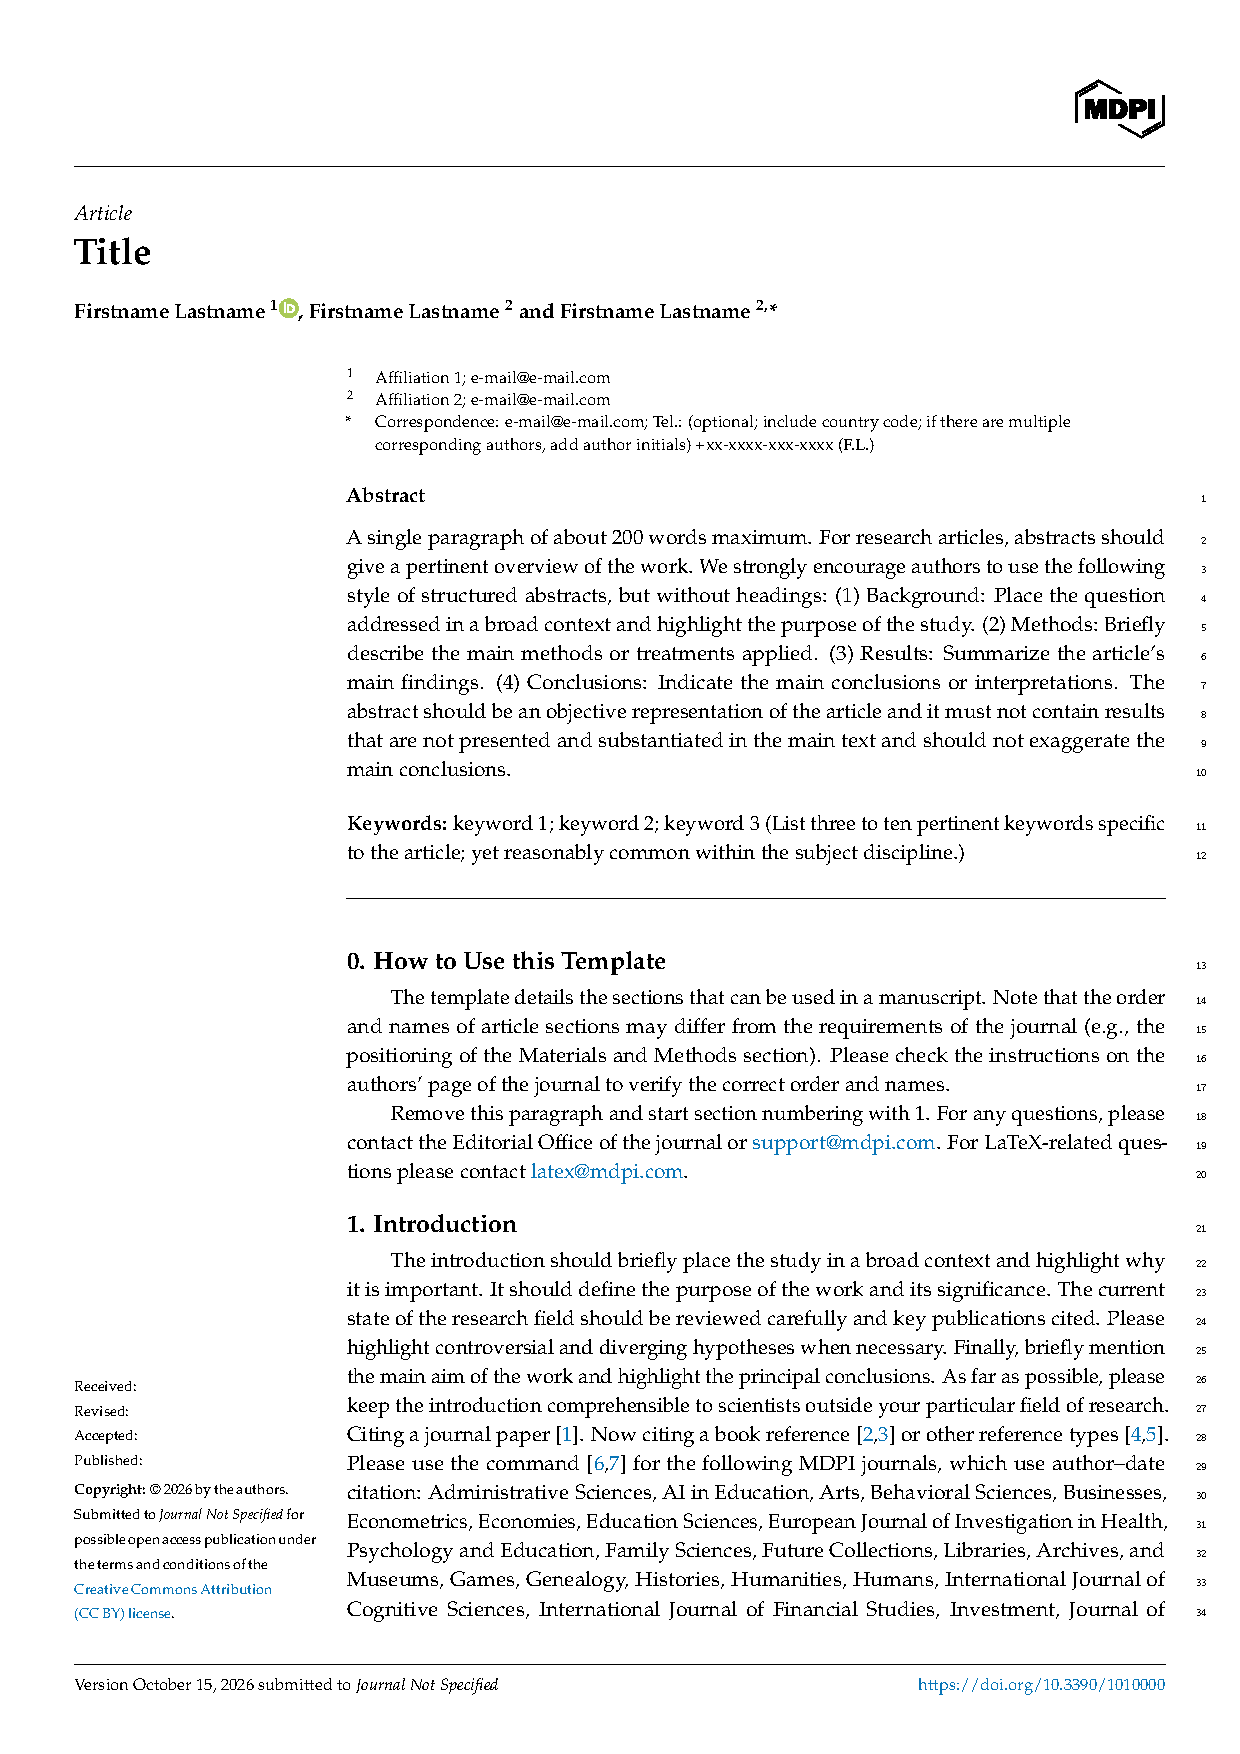
\includepdf[
        pages=-,
        scale=0.95,
        pagecommand={\thispagestyle{plain}}
    ]{papers/paper1.pdf}%
}{%
    \vspace*{2cm}
    \begin{center}
        \fbox{%
            \begin{minipage}{0.85\textwidth}
                \centering\vspace{1cm}
                \textbf{\large [Paper 1 PDF Pending: \texttt{papers/paper1.pdf}]}\\[0.5cm]
                \textit{The compiled PDF was not found in the \texttt{papers/} directory.}\\
                Link or upload the compiled PDF as \texttt{papers/paper1.pdf} to embed the complete publication.
                \vspace{1cm}
            \end{minipage}%
        }
    \end{center}
}

% Chapter 3: Publication 2 (Dissipative Strang Operator Splitting)
% ------------------------------------------------------------------------------
% CHAPTER 4: PAPER 3 (AAS 26-993: EMBEDDED AI ARCHITECTURE)
% ------------------------------------------------------------------------------
\chapter{High-Fidelity Semi-Symplectic Integration under Non-Conservative Forces}
\chaptermark{Semi-Symplectic Strang Splitting}
\label{ch:paper2}

\section*{Chapter Overview and Contextualization}
This chapter addresses the third specific objective of the doctoral research by embedding a multi-tier Artificial Intelligence (AI) architecture directly within the semi-symplectic propagation pipeline. This work synthesizes the methodology and findings published in the \textit{AAS/AIAA Astrodynamics Specialist Conference} (Paper AAS 26-993).

Although the hybrid Strang splitting integrator maintains numerical stability across 50,000 fragments, executing high-density operational tasks---such as pairwise conjunction screening and iterative inverse fragmentation targeting---introduces severe computational latency. Evaluating atmospheric drag using piecewise-exponential lookups introduces gradient discontinuities that perturb the numerical core, while all-on-all conjunction screening scales quadratically ($\mathcal{O}(N^2)$). Furthermore, solving the inverse problem of locating historical breakup coordinates is constrained by file I/O bottlenecks.

To resolve these challenges, this chapter establishes a three-phase AI ecosystem:
\begin{enumerate}
    \item A \textbf{PINN Thermospheric Surrogate} regularized by the differential hydrostatic equilibrium equation to deliver smooth, continuously differentiable density values across LEO.
    \item A \textbf{Spatial KD-Tree} that reduces pairwise distance searches to $\mathcal{O}(N \log N)$, combined with an \textbf{LSTM Sequence Classifier} that accurately identifies high-risk kinematic conjunctions amidst extreme class imbalance.
    \item A \textbf{PPO Reinforcement Learning Agent} connected to the C-compiled symplectic engine via a \texttt{ctypes} shared-memory pointer interface. Operating entirely within hardware RAM across 16 CPU cores, the agent generates 37~FPS, optimizing historical event coordinates without disk serialization overhead.
\end{enumerate}
Computational benchmarks confirm that the integrated AI-symplectic framework preserves the global $\mathcal{O}(N^{1.60})$ power-law scalability curve, providing a scalable computational engine for real-time space traffic coordination.

\newpage
% \includepdf[pages=-, scale=0.95, pagecommand={\thispagestyle{plain}}]{papers/AAS_26_993.pdf}

\clearpage

% Check if the compiled PDF exists; embed if found, display placeholder if missing
\IfFileExists{papers/paper2.pdf}{%
    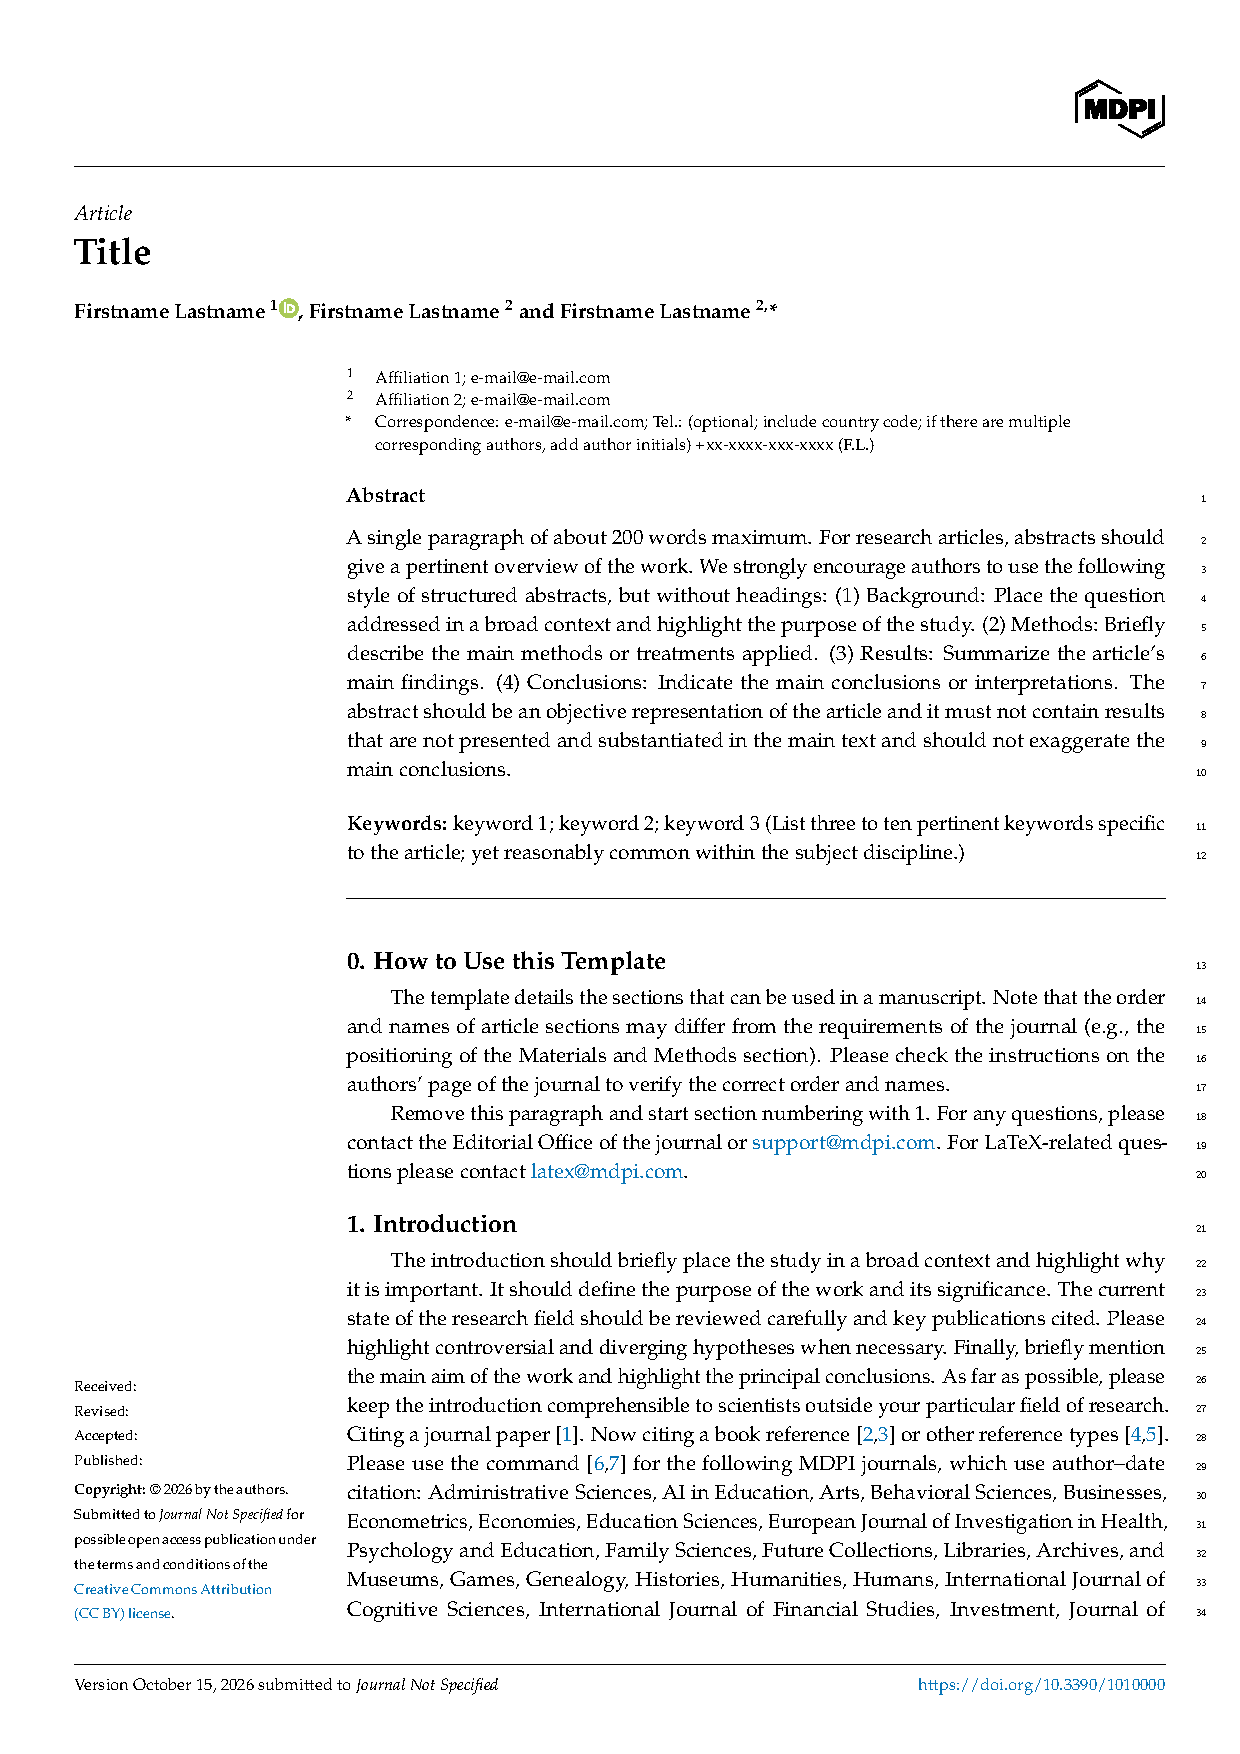
\includepdf[
        pages=-,
        scale=0.95,
        pagecommand={\thispagestyle{plain}}
    ]{papers/paper1.pdf}%
}{%
    \vspace*{2cm}
    \begin{center}
        \fbox{%
            \begin{minipage}{0.85\textwidth}
                \centering\vspace{1cm}
                \textbf{\large [Paper 2 PDF Pending: \texttt{papers/paper2.pdf}]}\\[0.5cm]
                \textit{The compiled PDF was not found in the \texttt{papers/} directory.}\\
                Link or upload the compiled PDF as \texttt{papers/paper2.pdf} to embed the complete publication.
                \vspace{1cm}
            \end{minipage}%
        }
    \end{center}
}

% Chapter 4: Publication 3 (AAS 26-993 / Embedded AI Ecosystem)
% ------------------------------------------------------------------------------
% CHAPTER 4: PAPER 3 (AAS 26-993: EMBEDDED AI ARCHITECTURE)
% ------------------------------------------------------------------------------
\chapter{Advanced Validation of a High-Fidelity Hybrid Symplectic Propagator for Massive Space Debris Fragmentation Analysis}
\chaptermark{Embedded AI for Debris Dynamics}
\label{ch:paper3}

\section*{Chapter Overview and Contextualization}
This chapter addresses the third specific objective of the doctoral research by embedding a multi-tier Artificial Intelligence (AI) architecture directly within the semi-symplectic propagation pipeline. This work synthesizes the methodology and findings published in the \textit{AAS/AIAA Astrodynamics Specialist Conference} (Paper AAS 26-993).

Although the hybrid Strang splitting integrator maintains numerical stability across 50,000 fragments, executing high-density operational tasks---such as pairwise conjunction screening and iterative inverse fragmentation targeting---introduces severe computational latency. Evaluating atmospheric drag using piecewise-exponential lookups introduces gradient discontinuities that perturb the numerical core, while all-on-all conjunction screening scales quadratically ($\mathcal{O}(N^2)$). Furthermore, solving the inverse problem of locating historical breakup coordinates is constrained by file I/O bottlenecks.

To resolve these challenges, this chapter establishes a three-phase AI ecosystem:
\begin{enumerate}
    \item A \textbf{PINN Thermospheric Surrogate} regularized by the differential hydrostatic equilibrium equation to deliver smooth, continuously differentiable density values across LEO.
    \item A \textbf{Spatial KD-Tree} that reduces pairwise distance searches to $\mathcal{O}(N \log N)$, combined with an \textbf{LSTM Sequence Classifier} that accurately identifies high-risk kinematic conjunctions amidst extreme class imbalance.
    \item A \textbf{PPO Reinforcement Learning Agent} connected to the C-compiled symplectic engine via a \texttt{ctypes} shared-memory pointer interface. Operating entirely within hardware RAM across 16 CPU cores, the agent generates 37~FPS, optimizing historical event coordinates without disk serialization overhead.
\end{enumerate}
Computational benchmarks confirm that the integrated AI-symplectic framework preserves the global $\mathcal{O}(N^{1.60})$ power-law scalability curve, providing a scalable computational engine for real-time space traffic coordination.

\newpage
% \includepdf[pages=-, scale=0.95, pagecommand={\thispagestyle{plain}}]{papers/AAS_26_993.pdf}

\clearpage

% Check if the compiled PDF exists; embed if found, display placeholder if missing
\IfFileExists{papers/paper2.pdf}{%
    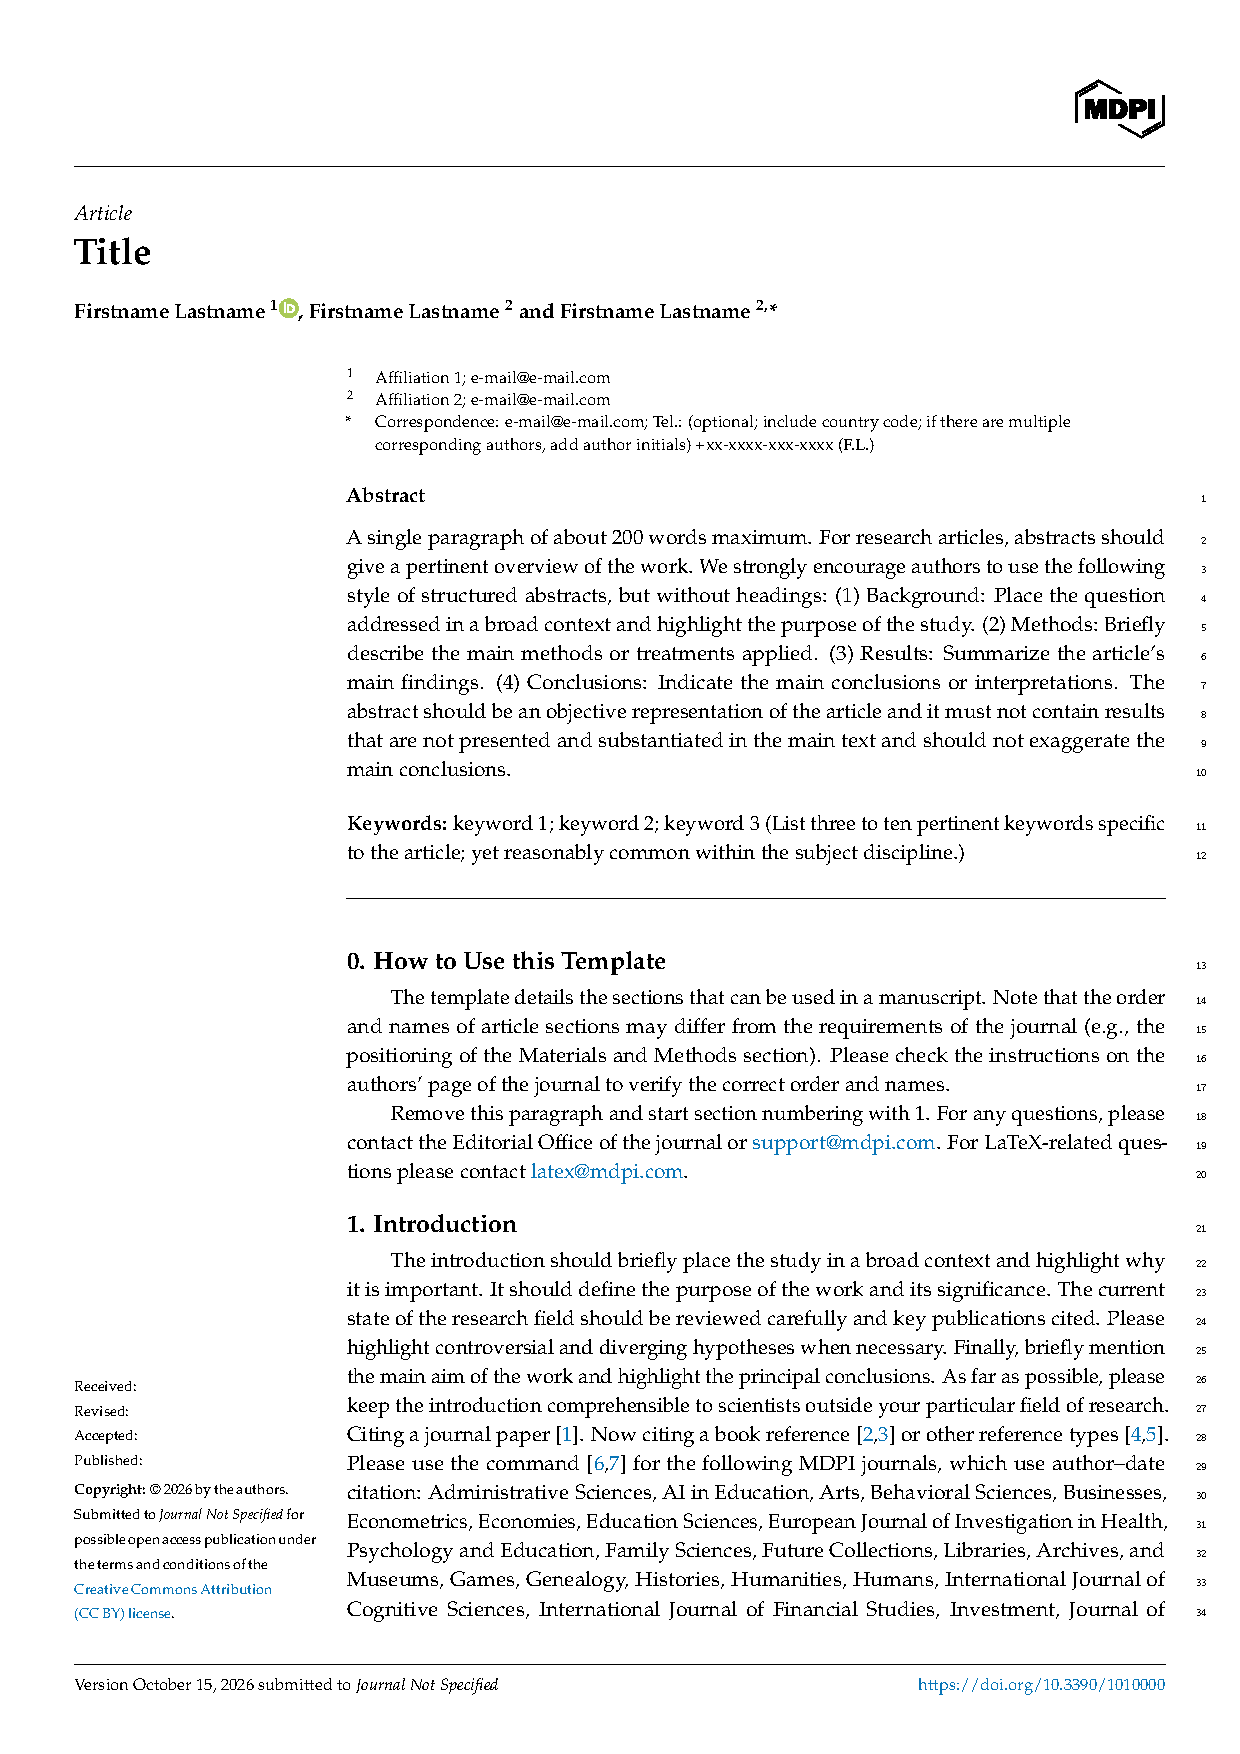
\includepdf[
        pages=-,
        scale=0.95,
        pagecommand={\thispagestyle{plain}}
    ]{papers/paper1.pdf}%
}{%
    \vspace*{2cm}
    \begin{center}
        \fbox{%
            \begin{minipage}{0.85\textwidth}
                \centering\vspace{1cm}
                \textbf{\large [Paper 3 PDF Pending: \texttt{papers/paper3.pdf}]}\\[0.5cm]
                \textit{The compiled PDF was not found in the \texttt{papers/} directory.}\\
                Link or upload the compiled PDF as \texttt{papers/paper3.pdf} to embed the complete publication.
                \vspace{1cm}
            \end{minipage}%
        }
    \end{center}
}

% Chapter 5: Global Discussion, Conclusions & Strategic Outlook
% ------------------------------------------------------------------------------
% CHAPTER 5: CONCLUSIONS AND FUTURE WORK
% ------------------------------------------------------------------------------
\chapter{Conclusions and Future Work}
\label{ch:conclusions}

\section{General Conclusions}
This doctoral dissertation successfully fulfilled its general objective by designing, implementing, and validating an AI-enhanced, high-fidelity hybrid semi-symplectic computational framework for simulating massive space debris fragmentation and orbital population dynamics in Low Earth Orbit. By bridging structure-preserving symplectic numerical integrators with advanced deep learning and reinforcement learning models, the research resolves the trade-off between long-term physical fidelity and computational scalability.

The fulfillment of the first specific objective established that symplectic $N$-body architectures natively eliminate secular mechanical energy drift in orbital mechanics. Validated in Chapter~\ref{ch:paper1}, the WHFast implementation preserved energy error bounds within $\vert{}\Delta E/E_0\vert{} \le 10^{-7}$ for 20,000 fragments under Earth's $J_2/J_4$ geopotential field, achieving sub-kilometer positional agreement with NASA's GMAT and demonstrating an empirical power-law scalability exponent of 1.60.

The second specific objective demonstrated that dissipative environmental forces can be integrated into symplectic algorithms without destroying their underlying geometric properties. As demonstrated in Chapter~\ref{ch:paper2}, the symmetric second-order Strang operator splitting sequence successfully decoupled conservative Hamiltonian gravity from non-conservative atmospheric drag and Solar Radiation Pressure. The model accurately reproduced secular nodal precession within 0.005\% of analytical theory across 50,000 fragments and captured the physical orbital sorting effect driven by variations in area-to-mass ratios.

Finally, the third specific objective demonstrated that localized artificial intelligence architectures can eliminate computational latency bottlenecks in space traffic management. As detailed in Chapter~\ref{ch:paper3}, embedding a Physics-Informed Neural Network (PINN) produced a $\mathcal{C}^\infty$-differentiable thermospheric density surrogate that eliminated table lookup discontinuities. Concurrently, spatial KD-Tree partitioning reduced conjunction screening complexity from $\mathcal{O}(N^2)$ to $\mathcal{O}(N \log N)$, enabling downstream LSTM sequence models to classify collision trajectories with high fidelity. Furthermore, coupling the C-compiled numerical engine with a Python PPO agent via a shared-memory \texttt{ctypes} interface enabled inverse fragmentation event reconstruction entirely within hardware RAM at 37~FPS.

In summary, the transition from pure symplectic $N$-body propagators to hybrid Strang-split formulations, culminating in an integrated AI-astrodynamics ecosystem, establishes a scalable, physically consistent computational tool for orbital debris forecasting and space traffic management.

\section{Specific Conclusions}

\paragraph{Performance of Symplectic $N$-Body Propagators (Objective 1):}
\begin{itemize}
    \item Symplectic integrators effectively prevent the accumulation of secular energy drift inherent to classical explicit numerical methods (such as Runge-Kutta and Cowell schemes) when modeling orbital mechanics over long durations.
    \item The WHFast symplectic solver maintained relative energy errors within $\vert{}\Delta E/E_0\vert{} \in [10^{-8}, 10^{-7}]$ across 24-hour simulations of 20,000 LEO fragments.
    \item Cross-validation against NASA's General Mission Analysis Tool (GMAT) demonstrated sub-kilometer positional agreement while maintaining an empirical computational scaling exponent of 1.60.
\end{itemize}

\paragraph{High-Fidelity Strang Operator Splitting (Objective 2):}
\begin{itemize}
    \item Second-order Strang splitting ($\Phi_P(\Delta t/2) \circ \Phi_G(\Delta t) \circ \Phi_P(\Delta t/2)$) successfully isolates non-conservative dissipative forces into symmetric half-step kicks, preventing numerical dissipation from degrading the primary symplectic gravitational flow.
    \item Constant step sizes ($\Delta t = 10$~s) ensure that the numerical flow advances via a single symplectic mapping, avoiding the quadratic error growth associated with variable-step symplectic schemes.
    \item The hybrid model reproduced secular nodal precession within 0.005\% of analytical theory and simulated physical orbital sorting across 50,000 fragments with varying area-to-mass ratios ($A/m$).
\end{itemize}

\paragraph{Embedded Artificial Intelligence Integration (Objective 3):}
\begin{itemize}
    \item Physics-Informed Neural Networks regularized by the differential hydrostatic equilibrium equation provide continuous, $\mathcal{C}^\infty$-differentiable atmospheric density fields, eliminating numerical gradient jumps typical of piecewise lookups.
    \item Spatial KD-Tree domain decomposition reduces conjunction screening complexity from $\mathcal{O}(N^2)$ to $\mathcal{O}(N \log N)$, enabling LSTM sequence classifiers to evaluate kinematic arcs with high recall amidst severe class imbalance.
    \item Establishing a direct \texttt{ctypes} foreign function interface between C and Python eliminates disk I/O bottlenecks, enabling parallel PPO reinforcement learning rollouts in RAM at 37~FPS across 16 CPU cores for autonomous breakup reconstruction.
    \item Benchmarking confirmed that the integrated AI-symplectic framework preserves the global $\mathcal{O}(N^{1.60})$ power-law scalability curve.
\end{itemize}

\section{Future Work}
Based on the findings and computational trade-offs identified throughout this research, several directions are proposed for future investigation:
\begin{itemize}
    \item \textbf{Distributed HPC Cluster Scaling:} Transition the current shared-memory OpenMP architecture to distributed multi-node Graphics Processing Unit (GPU) clusters (utilizing Message Passing Interface (MPI) and Compute Unified Device Architecture (CUDA)) to scale PPO optimization horizons beyond $10^7$ timesteps, driving inverse tracking residuals down to sub-kilometer accuracy.
    \item \textbf{Cislunar and Multi-Body Gravity Expansion:} Extend the symplectic gravitational core to incorporate multi-body third-body perturbations (Sun and Moon) and non-spherical lunar gravity fields, utilizing spatial-temporal Graph Neural Networks (GNNs) or Attention Transformers to assess cislunar fragmentation dynamics.
    \item \textbf{Autonomous Time-Reversible Inversion:} Exploit the geometric time-reversibility of symplectic maps by executing negative time-step integrations ($\Delta t < 0$), allowing reinforcement learning agents to trace dispersed debris clouds backward through perturbed thermospheric regimes to identify parent satellite breakups autonomously.
    \item \textbf{Hardware-in-the-Loop Validation:} Implement the trained PINN surrogates and KD-Tree/LSTM models on embedded radiation-hardened spacecraft processors to evaluate onboard autonomous collision avoidance and decentralized space traffic coordination.
\end{itemize}

\clearpage

\clearpage

% ==============================================================================
% MASTER BIBLIOGRAPHY
% ==============================================================================
\backmatter
\addcontentsline{toc}{chapter}{Bibliography}
\bibliographystyle{IEEEtran}
%\nocite{*}
\bibliography{references}

\end{document}